\graphicspath{ {images/datatables/} }
\subsection{Работа с табличными представлениями} \label{sec:datatables}

Табличные данные в АРМ вуза имеют унифицированное представление и содержат следующие элементы управления:
\begin{itemize}
	\item Выбор количества записей на странице \vcenteredinclude[height=25px]{page_count}
	\item Кнопка экспорта текущей выборки в CSV-файл \vcenteredinclude[height=25px]{csv_export}
	\item Кнопка вызова диалога фильтрации \vcenteredinclude[height=25px]{filter}
	\item Строка поиска \vcenteredinclude[height=25px]{search}
	\item Элемент постраничной навигации \vcenteredinclude[height=25px]{pagination}
\end{itemize}

Пример табличных данных приведён на рис.~\ref{img:datatables:dt}

\begin{figure}[H]
	\center{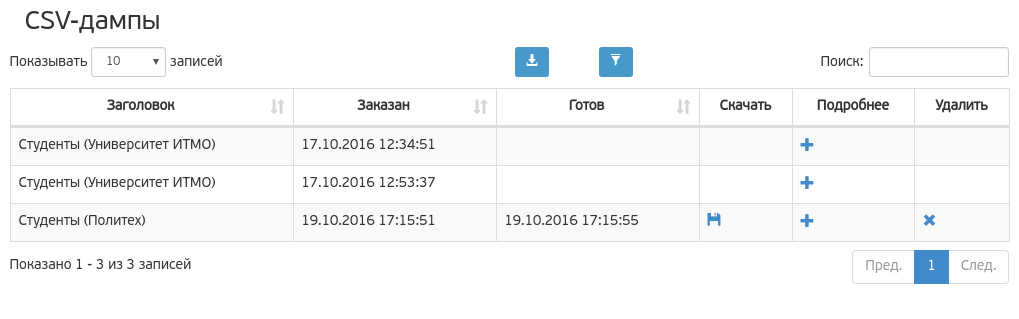
\includegraphics[width=1\linewidth]{dt}}
	\caption{Пример табличных данных}
	\label{img:datatables:dt}
\end{figure}

\subsubsection{Сортировка}

Для большинства столбцов доступна сортировка таблицы по их содержимому. Для некоторых столбцов сортировка недоступна
либо ввиду бессмысленности (в каждой ячейке находится одинаковая иконка), либо ввиду технических ограничений.
Если для столбца доступна сортировка, то в его заголовке есть значок \vcenteredinclude[height=25px]{sort_icon}.
Если таблица отсортирована по какому"=либо столбцу по убыванию, то в его заголовке есть значок \vcenteredinclude[height=25px]{sort_icon_desc},
по возрастанию "--- \vcenteredinclude[height=25px]{sort_icon_asc}.

Для сортировки по какому"=либо столбцу необходимо нажать на его заголовок. Для переключения режима сортировки <<по возрастанию>> "--- <<по убыванию>>,
необходимо повторно нажимать на заголовок того же столбца. Для сортировки по нескольким столбцам таблицы необходимо выбрать первый столбец обычным способом,
а затем нажимать на последующие при нажатой клавише \keys{\shift\ Shift}.

\subsubsection{Поиск}

В таблицах доступен поиск по содержимому всех столбцов. Для поиска текста в таблице необходимо ввести этот текст в строку поиска. Если требуется 
найти текст из нескольких слов в одном столбце, необходимо заключить этот текст в двойные или одинарные кавычки. Поиск осуществляется по мере набора текста.

\subsubsection{Фильтрация}

Во всех таблицах присутствует форма фильтрации, которую можно вызвать нажатием кнопки \vcenteredinclude[height=25px]{filter}. Для числовых полей и полей с датой в форме фильтрации предусмотрена фильтрация по диапазону. После применения фильтрации рядом с кнопкой \vcenteredinclude[height=25px]{filter} появляется кнопка \vcenteredinclude[height=25px]{filter_clear_button}.
При нажатии на неё все фильтры из формы фильтрации очищаются и таблица обновляется. 

\subsubsection{Выгрузка в CSV}

Для выгрузки табличных данных в формате CSV требуется нажать кнопку \vcenteredinclude[height=25px]{csv_export}. Данные из таблиц
сохраняются в файл в формате CSV, который может быть открыт в Microsoft Excel или LibreOffice Calc. Сортировка, фильтрация и строка
поиска учитываются при выгрузке. Если число записей менее 300, то пользователю сразу будет предложено скачать выходной файл, в противном случае файл будет выслан пользователю по почте и появится в разделе <<Мои выгрузки>>
(см.\ подраздел~\ref{sec:csv_dumps}), пользователю при этом показывается соответствующее сообщение.
